\documentclass[]{article}
\usepackage{lmodern}
\usepackage{amssymb,amsmath}
\usepackage{ifxetex,ifluatex}
\usepackage{fixltx2e} % provides \textsubscript
\ifnum 0\ifxetex 1\fi\ifluatex 1\fi=0 % if pdftex
  \usepackage[T1]{fontenc}
  \usepackage[utf8]{inputenc}
\else % if luatex or xelatex
  \ifxetex
    \usepackage{mathspec}
  \else
    \usepackage{fontspec}
  \fi
  \defaultfontfeatures{Ligatures=TeX,Scale=MatchLowercase}
\fi
% use upquote if available, for straight quotes in verbatim environments
\IfFileExists{upquote.sty}{\usepackage{upquote}}{}
% use microtype if available
\IfFileExists{microtype.sty}{%
\usepackage{microtype}
\UseMicrotypeSet[protrusion]{basicmath} % disable protrusion for tt fonts
}{}
\usepackage[margin=1in]{geometry}
\usepackage{hyperref}
\hypersetup{unicode=true,
            pdftitle={Unveiling the ecosystem of science},
            pdfauthor={Nicolas Robinson-Garcia},
            pdfborder={0 0 0},
            breaklinks=true}
\urlstyle{same}  % don't use monospace font for urls
\usepackage{longtable,booktabs}
\usepackage{graphicx,grffile}
\makeatletter
\def\maxwidth{\ifdim\Gin@nat@width>\linewidth\linewidth\else\Gin@nat@width\fi}
\def\maxheight{\ifdim\Gin@nat@height>\textheight\textheight\else\Gin@nat@height\fi}
\makeatother
% Scale images if necessary, so that they will not overflow the page
% margins by default, and it is still possible to overwrite the defaults
% using explicit options in \includegraphics[width, height, ...]{}
\setkeys{Gin}{width=\maxwidth,height=\maxheight,keepaspectratio}
\IfFileExists{parskip.sty}{%
\usepackage{parskip}
}{% else
\setlength{\parindent}{0pt}
\setlength{\parskip}{6pt plus 2pt minus 1pt}
}
\setlength{\emergencystretch}{3em}  % prevent overfull lines
\providecommand{\tightlist}{%
  \setlength{\itemsep}{0pt}\setlength{\parskip}{0pt}}
\setcounter{secnumdepth}{0}
% Redefines (sub)paragraphs to behave more like sections
\ifx\paragraph\undefined\else
\let\oldparagraph\paragraph
\renewcommand{\paragraph}[1]{\oldparagraph{#1}\mbox{}}
\fi
\ifx\subparagraph\undefined\else
\let\oldsubparagraph\subparagraph
\renewcommand{\subparagraph}[1]{\oldsubparagraph{#1}\mbox{}}
\fi

%%% Use protect on footnotes to avoid problems with footnotes in titles
\let\rmarkdownfootnote\footnote%
\def\footnote{\protect\rmarkdownfootnote}

%%% Change title format to be more compact
\usepackage{titling}

% Create subtitle command for use in maketitle
\newcommand{\subtitle}[1]{
  \posttitle{
    \begin{center}\large#1\end{center}
    }
}

\setlength{\droptitle}{-2em}

  \title{Unveiling the ecosystem of science}
    \pretitle{\vspace{\droptitle}\centering\huge}
  \posttitle{\par}
    \author{Nicolas Robinson-Garcia}
    \preauthor{\centering\large\emph}
  \postauthor{\par}
      \predate{\centering\large\emph}
  \postdate{\par}
    \date{February 19, 2019}


\begin{document}
\maketitle

Introduction and lit review should lead to the model we propose. Hence
all aspects of the model should be reviewed in the paper. Maybe more
than a literature review is an Antecedents, or it is more than one
section.

\hypertarget{introduction}{%
\subsection{1. Introduction}\label{introduction}}

The ecosystem of science is defined as a system with interconnected
entities integrated in a larger social system with which a bidirectional
influence is exerted. Scientists, as drivers of the research enterprise,
are immersed in an increasingly diverse set of tasks and activities with
the purpose of producing, communicating and transferring knowledge to
society. This involves a series of skills which go beyond their
intellectual or technical capabilities. These additional tasks relate to
each of the activities they are involved in: production, communication
and transference of new knowledge. They must distribute tasks and
specialize, collaborate with their peers, train younger scholars and
build research teams to enhance their production capabilities. They must
interact and engage with non-academic actors to identify gaps of
knowledge, apply their research output on societal challenges and
communicate their findings in a responsible and efficient manner.

These different activities are rarely undertaken by the same individual.
There is distribution of roles, converting research into a collaborative
enterprise, where different profiles of researchers emanate from their
specialization on specific roles. Furthermore, individuals are involved
in different roles depending on their career stage, the characteristics
of their research field or the peers with whom they collaborate. While a
senior scientist will be involved in PhD supervision, research
assistants may undertake data collection tasks. Historians may not focus
on knowledge transference as much and civil engineers but might engage
on social outreach. A statistician may be giving methodological support
when collaborating with physicians but might be involved in theoretical
discussions when collaborating with mathematicians. In all, these roles
are not fixed and can evolve with time and change due to context.

This diversification of roles affects authorship and acknowledgement of
research outputs, favoring certain profiles over others. Evaluation
schemes are mostly (if not exclusively) focused on research outputs and
citation impact. This has led to a series of claims as to how current
evaluation schemes are threatening diversity of profiles and roles, and
ultimately, the ecosystem of science. These claims are discussed below.

\textbf{Claim 1: Evaluation schemes rely solely on journal publication
and citation-based indicators.}

\begin{itemize}
\tightlist
\item
  What do evaluation systems state they want from individuals?
\item
  What is their actual criteria?
\item
  Supporting evidence: DORA Declaration
\end{itemize}

\textbf{Claim 2: Publications offer a partial view of researchers'
outcomes.}

\begin{itemize}
\tightlist
\item
  What do researchers do?
\item
  How they organize their time?
\item
  Which are their outcomes?
\end{itemize}

\textbf{Claim 3: Invisible profiles are becoming more necessary than
ever but are being kicked out of the system.}

\begin{itemize}
\tightlist
\item
  How do they distribute tasks?
\item
  How do they negotiate authorship?
\item
  How do they allocate credit and prestige
\item
  Supporting evidence: Milojevic et al.~PNAS (2018) publication.
\end{itemize}

\hypertarget{lit-review}{%
\subsection{2. Lit review}\label{lit-review}}

\hypertarget{stratification-and-diversity-of-scientific-profiles}{%
\subsection{Stratification and diversity of scientific
profiles}\label{stratification-and-diversity-of-scientific-profiles}}

Examples of dimensions can be given from the book by Bastow, Tinkler \&
Dunleavy (2014)

Bozeman, Dietz \& Gaughan (2001) present their evaluation model at the
individual level as follows:

\begin{itemize}
\tightlist
\item
  Internal resources: cognitive skills (this can be criticized as it is
  impossible to operationalize as they present it i.e., ability to
  synthesize), S\&T knowledge and context skills (learnt through
  experience). The authors indicate that each resource may have n
  dimensions.
\item
  S\&T Capital: Which has to do with the network of scientists and the
  intrinsic value they have as well as the role the individual plays in
  such network
\item
  S\&T Human Capital and Life Cycles: The authors recognize that
  researchers' profile will be different at different stages of their
  career.
\item
  Corley et al (2017) introduce a cultural dimension to the model which
  refers to variables such as gender, nationality, race, discipline or
  socio-economic status.
\end{itemize}

ACUMEN presents a portfolio, a kind of CV format designed for assessing
individual performance. It combines qualitative and quantitative
information. It offers space for a narrative where an individual tells
her own story. It then distinguishes between three aspects of an
academic's career: expertise (methods, areas of theory, etc.), outputs
(publications, patents, etc.) and impacts (citations, awards, etc.).
Furthermore, it includes an individual's age. For these three aspects it
includes quantitative indicators. The perspective here is that
individuals report their CV and the ACUMEN portfolio basically
structures and offers recommendations on how this should be provided.
Other than that it does not give clear indications on how the assessment
should be performed, it seems to rely on experts' judgment. Look into
Whitley Look into Evaluative Inquiry

\hypertarget{effects-of-evaluation-on-research-careers-some-evidences}{%
\subsubsection{Effects of evaluation on research careers: Some
evidences}\label{effects-of-evaluation-on-research-careers-some-evidences}}

Abramo, G., D'Angelo, C. A., \& Rosati, F. (2015). The determinants of
academic career advancement: Evidence from Italy. Science and Public
Policy, 42(6), 761-774. \url{https://doi.org/10.1093/scipol/scu086}

Luukkonen, T., \& Thomas, D. A. (2016). The `Negotiated Space' of
University Researchers' Pursuit of a Research Agenda. Minerva, 54(1),
99-127. \url{https://doi.org/10.1007/s11024-016-9291-z}

\hypertarget{career-trajectories}{%
\paragraph{Career trajectories}\label{career-trajectories}}

Stephan \& Levin -\textgreater{} In terms of productivity peaks and
decline

Laudel, G., Bielick, J., \& Gläser, J. (2018). `Ultimately the question
always is: ``What do I have to do to do it right?''\,' Scripts as
explanatory factors of career decisions. Human Relations,
0018726718786550. \url{https://doi.org/10.1177/0018726718786550}

\hypertarget{evaluation-models-of-scientific-activity}{%
\subsubsection{Evaluation models of scientific
activity}\label{evaluation-models-of-scientific-activity}}

\begin{longtable}[]{@{}llll@{}}
\toprule
\begin{minipage}[b]{0.24\columnwidth}\raggedright
Evaluation model\strut
\end{minipage} & \begin{minipage}[b]{0.23\columnwidth}\raggedright
Output/outcome\strut
\end{minipage} & \begin{minipage}[b]{0.25\columnwidth}\raggedright
Unit of analysis\strut
\end{minipage} & \begin{minipage}[b]{0.16\columnwidth}\raggedright
References\strut
\end{minipage}\tabularnewline
\midrule
\endhead
\begin{minipage}[t]{0.24\columnwidth}\raggedright
Bibliometric assessment\strut
\end{minipage} & \begin{minipage}[t]{0.23\columnwidth}\raggedright
Production and impact\strut
\end{minipage} & \begin{minipage}[t]{0.25\columnwidth}\raggedright
Scalable\strut
\end{minipage} & \begin{minipage}[t]{0.16\columnwidth}\raggedright
\strut
\end{minipage}\tabularnewline
\begin{minipage}[t]{0.24\columnwidth}\raggedright
Economic analysis\strut
\end{minipage} & \begin{minipage}[t]{0.23\columnwidth}\raggedright
\strut
\end{minipage} & \begin{minipage}[t]{0.25\columnwidth}\raggedright
\strut
\end{minipage} & \begin{minipage}[t]{0.16\columnwidth}\raggedright
\strut
\end{minipage}\tabularnewline
\begin{minipage}[t]{0.24\columnwidth}\raggedright
Knowledge value alliances\strut
\end{minipage} & \begin{minipage}[t]{0.23\columnwidth}\raggedright
\strut
\end{minipage} & \begin{minipage}[t]{0.25\columnwidth}\raggedright
Communities of scholars (e.g., labs)\strut
\end{minipage} & \begin{minipage}[t]{0.16\columnwidth}\raggedright
Bozeman \& Rogers\strut
\end{minipage}\tabularnewline
\begin{minipage}[t]{0.24\columnwidth}\raggedright
Research portfolios\strut
\end{minipage} & \begin{minipage}[t]{0.23\columnwidth}\raggedright
Journal articles?\strut
\end{minipage} & \begin{minipage}[t]{0.25\columnwidth}\raggedright
\strut
\end{minipage} & \begin{minipage}[t]{0.16\columnwidth}\raggedright
Wallace \& Rafols, 2015\strut
\end{minipage}\tabularnewline
\begin{minipage}[t]{0.24\columnwidth}\raggedright
Productive interactions\strut
\end{minipage} & \begin{minipage}[t]{0.23\columnwidth}\raggedright
Process-oriented\strut
\end{minipage} & \begin{minipage}[t]{0.25\columnwidth}\raggedright
Research projects\strut
\end{minipage} & \begin{minipage}[t]{0.16\columnwidth}\raggedright
Spaape \& van Drooge, 2011\strut
\end{minipage}\tabularnewline
\begin{minipage}[t]{0.24\columnwidth}\raggedright
S\&T Human Capital\strut
\end{minipage} & \begin{minipage}[t]{0.23\columnwidth}\raggedright
\strut
\end{minipage} & \begin{minipage}[t]{0.25\columnwidth}\raggedright
Scalable\strut
\end{minipage} & \begin{minipage}[t]{0.16\columnwidth}\raggedright
Bozeman, Dietz \& Gaughan, 2001\strut
\end{minipage}\tabularnewline
\bottomrule
\end{longtable}

\hypertarget{methodological-framework}{%
\subsection{3. Methodological
framework}\label{methodological-framework}}

\hypertarget{evaluative-dimensions}{%
\subsubsection{Evaluative dimensions}\label{evaluative-dimensions}}

\hypertarget{scientific-engagement}{%
\paragraph{Scientific engagement}\label{scientific-engagement}}

Collaboration ties and diversity (number of unique collaborators and
intensity), position in network, (co-authorship, acknowledgment, etc.),
strength of tie?, interdisciplinarity, application of research, member
of committees, reviewer, etc. Social engagement Non-academic
collaboration ties (either through publications or not i.e., reference
patterns), some altmetric indicators (policy briefs but also maybe
twitter classes? Or potentially Ed's ABC score), spin-offs,
Capacity-building Productivity, leadership, independence, scientific
impact, funding Trajectory/Background? Geographic mobility, cognitive
mobility, sectoral mobility (These last three could be seen not as
attributes to the researcher but their capacity to work with diverse
people), career status Research practices (Cross-sectoral) OA
publications, data sharing, outreach (e.g., The Conversation, blogging,
tweeting), publication of working papers, proceedings, mentoring Some
references Alperin, J. P., Nieves, C. M., Schimanski, L., Fischman, G.
E., Niles, M. T., \& McKiernan, E. C. (2018). How significant are the
public dimensions of faculty work in review, promotion, and tenure
documents? Recuperado de
\url{https://hcommons.org/deposits/item/hc:21015/} July 3rd,
researchers, 2018\textbar{}Early career, education, H., science, O.,
evaluation, R., \& Comment, R. policy\textbar{}1. (2018, julio 3).
Making research evaluation processes in Europe more transparent.
Recuperado 20 de febrero de 2019, de
\url{https://blogs.lse.ac.uk/impactofsocialsciences/2018/07/03/making-research-evaluation-processes-in-europe-more-transparent/}
Schimanski, L. A., \& Alperin, J. P. (2018). The evaluation of
scholarship in academic promotion and tenure processes: Past, present,
and future. F1000Research, 7, 1605.
\url{https://doi.org/10.12688/f1000research.16493.1}

\hypertarget{confounding-effects}{%
\paragraph{Confounding effects}\label{confounding-effects}}

\hypertarget{personal-features}{%
\paragraph{Personal features}\label{personal-features}}

Order dimensions from time independent to dependent. Features within
dimensions

\hypertarget{results}{%
\subsection{4. Results}\label{results}}

\begin{itemize}
\tightlist
\item
  Showcase dimensions for research teams or labs -\textgreater{}
  Internal organization and division of labor
\item
  Showcase dimensions life cycles -\textgreater{} Different stages in
  career
\item
  Attribution Plos One -\textgreater{} Scientific engagement
\item
  Differences on profiles by fields.
\item
  Agencies
\end{itemize}

\pagebreak

\hypertarget{codebook}{%
\section{Codebook}\label{codebook}}

Here I describe the selection of case studies and the data retrieval
process and description of sources. The purpose of this is to show that
1) there are indeed a variety of different profiles, 2) these profiles
co-exist and complement each other, 3) the diversity and typologies of
profiles is field dependent, 4) personal features are key to understand
this diversity. Here we emphasize two specific personal features: age
and gender. Some of the research questions that could be answered
descriptively are the following:

\begin{enumerate}
\def\labelenumi{\arabic{enumi}.}
\tightlist
\item
  \emph{Is there team science?}
\end{enumerate}

\begin{enumerate}
\def\labelenumi{\roman{enumi}.}
\tightlist
\item
  \emph{Are these teams stable over time?} Some data that could be
  retrieved from WoS
\end{enumerate}

\begin{verbatim}
-   Cluster_id
-   All classic bibliometric indicators
-   Number of collaborators from same institution
-   Number of external collaborators
-   Number of collaborators from same institution by publication
-   Number of external collaborators by publication
\end{verbatim}

\begin{enumerate}
\def\labelenumi{\roman{enumi}.}
\setcounter{enumi}{1}
\tightlist
\item
  \emph{Is there activity visible through co-authorship?} Check groups
  identified with manual checking in the web and maybe interviews
\end{enumerate}

\begin{enumerate}
\def\labelenumi{\arabic{enumi}.}
\setcounter{enumi}{1}
\tightlist
\item
  \emph{Do research teams operate in a coordinated way?} Here it would
  be interesting to understand dependence relationship. Nederhof \& van
  Raan (1993) refer to the star effects as what happens when a PI
  retires and the research group disappears. Here we should go beyond
  bibliometrics and see if there is someone in charge of the funding,
  someone of hiring and finding opportunities, someone who is more of a
  public face, etc. Also it would be interesting to use network analysis
  to determine authorities, hubs, etc. and contrast with their judgment.
  Some variables from WoS and interivews plus manually cheking:
  authorship position (WoS); acknowledgments data (WoS); clusters from
  Ludo's subject classification to identify areas of specialization per
  subject (WoS); social media activity; Google Scholar data.
\end{enumerate}

\begin{enumerate}
\def\labelenumi{\roman{enumi}.}
\tightlist
\item
  \emph{Do they have a common research agenda?}
\item
  \emph{How is this agenda established?}
\end{enumerate}

\begin{enumerate}
\def\labelenumi{\arabic{enumi}.}
\setcounter{enumi}{2}
\tightlist
\item
  \emph{How does team science affect individual trajectories?}
\end{enumerate}

\begin{enumerate}
\def\labelenumi{\roman{enumi}.}
\tightlist
\item
  \emph{How is credit shared?}
\item
  \emph{What is the relation between the role exerted and academic
  status?} A cohort analysis?
\item
  \emph{How is continuity of supporting scientists ensured?} Probably
  also from interviews. How do scholars change from institution or are
  maintained if they are not able to `make the next step'.
\end{enumerate}

\hypertarget{selection-of-case-studies}{%
\subsection{Selection of case studies}\label{selection-of-case-studies}}

The identification of research groups is done bibliometrically and based
on Web of Science publications. For this I have selected all
publications between 2008 and 2017 by LUMC, Leiden University or TU
Delft. The following table includes some descriptives. Here I must note
that researchers belonging to institutions are not based on the specific
affiliation linkage of docs (which uses the Leiden Ranking affiliation
already cleaned up), but based on \texttt{cluster\_id} with either of
the three institutions as their main or alternative address. This should
be checked to see if there is a way to link to the \texttt{cluster\_id}
organizations to the cleaned affiliations from Leiden Ranking. I had to
clean up this data myself. In any case this should not be a concern for
the selection of case studies.

\begin{longtable}[]{@{}lccc@{}}
\toprule
& TU Delft & Leiden Univ & LUMC\tabularnewline
\midrule
\endhead
Publications & 24,233 & 49,149 & 3,188\tabularnewline
Researchers & 9,975 & 14,116 & 279\tabularnewline
Collaborators & 34,409 & 117,307 & 14,153\tabularnewline
Mean au/p & 4.7 & 9.6 & 10.1\tabularnewline
Median au/p & 4 & 6 & 8\tabularnewline
Sd au/p & 5.4 & 31.5 & 18.7\tabularnewline
\bottomrule
\end{longtable}

The next figure shows the distribution of papers based on the number of
authors by paper (A) and the thematic profile of each of the three
institutions. Leiden University is the largest of the three institutions
with a more comprehensive portfolio, although mostly focues on
Biomedical Sciences and Social Sciences. This focus on biomedical
sciences is obviously more noticeable in the case of LUMC, although it
still has some pubications in fields of the social sciences, mostly
related with Public Health. Finally, TU Delft shows a profile focused on
Phisics, Engineering and Mathematics. While there might be an overlap
between LUMC and Leiden University, the high preponderance of biomedical
literature might also be due to a close relation between these
universities.

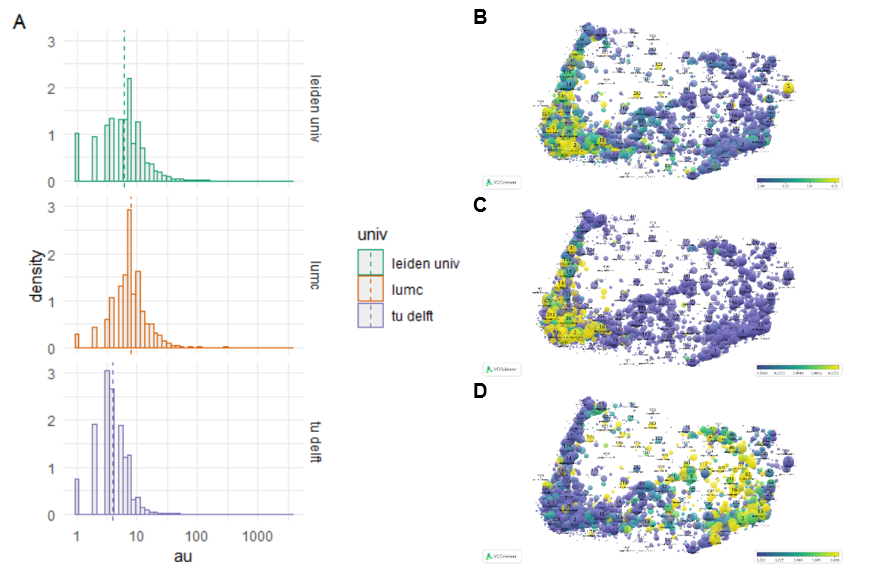
\includegraphics[width=7.14in]{figs/histogram-profiles}

Six case studies will be selected. Three for each university and two by
field. The purpose of this is not only to identify differences by
discipline but also by institutional type. The fields are:

\begin{enumerate}
\def\labelenumi{\arabic{enumi}.}
\tightlist
\item
  Physics and Engineering
\item
  Social Sciences and Humanities
\item
  Biomedical Sciences
\end{enumerate}

Following I include the collaboration networks for each university and
field. I have included a threshold of at least 10 publications by
\texttt{cluster\_id}, filtered by the giant component and calculated the
betweenness centrality of each node. I have selected as seed researcher
the one with the highest centrality.

\hypertarget{physics-engineering}{%
\subsubsection{Physics \& Engineering}\label{physics-engineering}}

\hypertarget{tu-delft}{%
\paragraph{1. TU Delft}\label{tu-delft}}

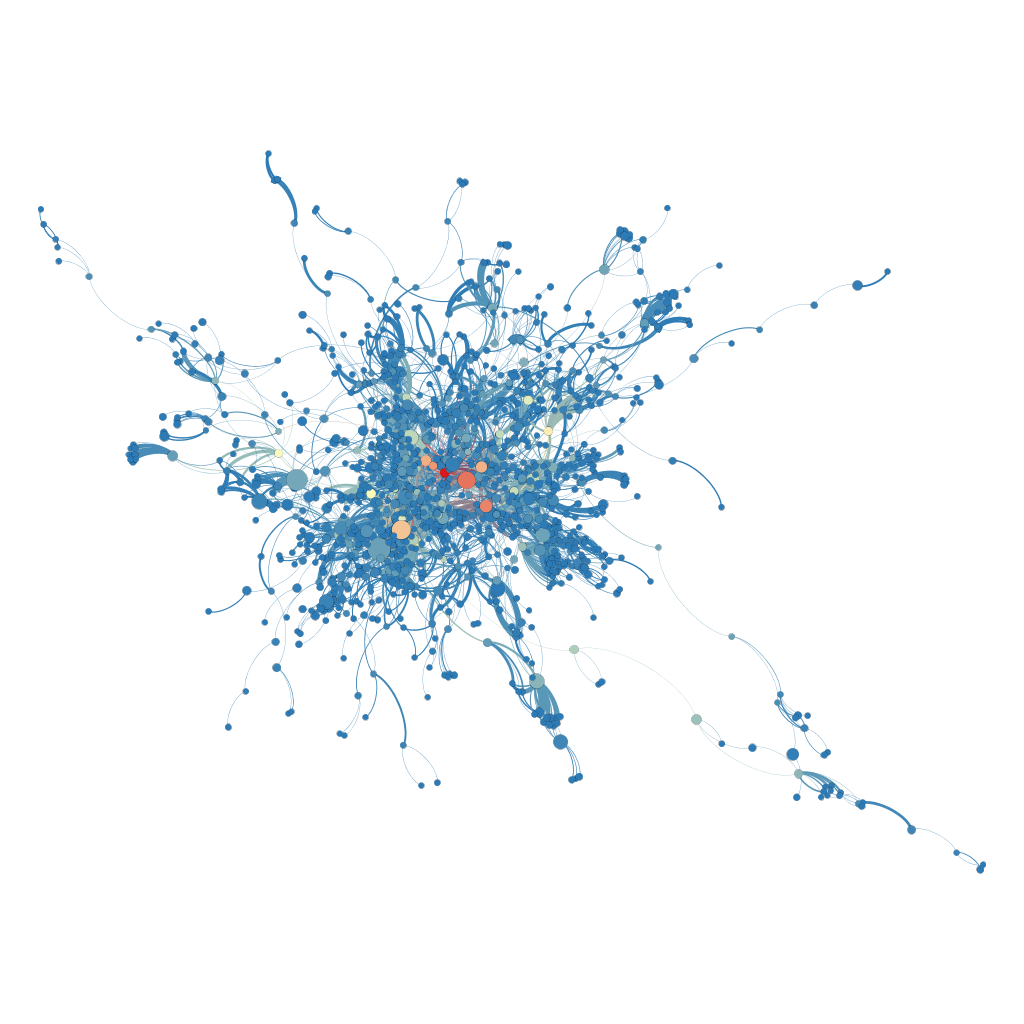
\includegraphics[width=8.19in]{figs/tu_phys_betweenness}

\emph{Notes:}

\begin{itemize}
\tightlist
\item
  1260 nodes (21.9\% visible); 4702 edges (27.1\% visible).
\item
  \texttt{cluster\_id} with highest betweenness = 33800547; Betweenness
  centrality: 0.11; Total publications = 159; Age = 32
\item
  Name: Frans D. Tichelaar; First year: 1986; Last year: 2018
\item
  PURE:
  \url{https://pure.tudelft.nl/portal/en/persons/fd-tichelaar(56299c58-b6ec-478b-b188-b8744b69d954).html}
\item
  Institution: \url{http://nchrem.nl/people/dr-ir-f-d-tichelaar-frans/}
\end{itemize}

\hypertarget{leiden-univ}{%
\paragraph{2. Leiden Univ}\label{leiden-univ}}

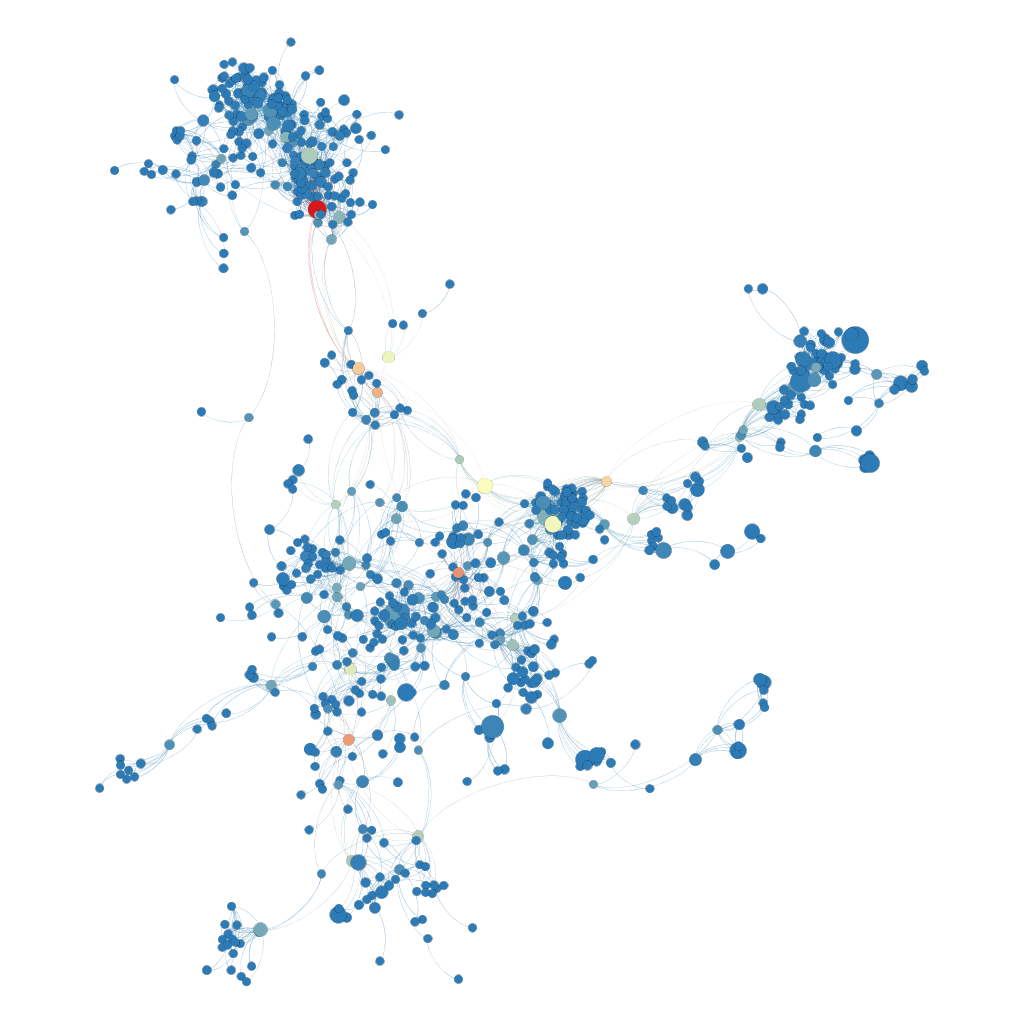
\includegraphics[width=3.41in]{figs/lu_phys_betweenness}

\emph{Notes:}

\begin{itemize}
\tightlist
\item
  765 nodes (35.1\% visible); 3409 edges (40.6\% visible).
\item
  \texttt{cluster\_id} with highest betweenness = 25501410; Betweenness
  centrality: 0.23; Total publications = 590; Age = 38
\item
  Name: Ewine F. van Dishoeck; First year: 1980; Last year: 2018
\item
  Institution:
  \url{https://local.strw.leidenuniv.nl/people/touchscreen2/persinline.php?id=16}
\item
  Personal website: \url{https://home.strw.leidenuniv.nl/~ewine/}
\end{itemize}

\hypertarget{biomedical-and-health-sciences}{%
\subsubsection{Biomedical and Health
Sciences}\label{biomedical-and-health-sciences}}

\hypertarget{tu-delft-1}{%
\paragraph{1. TU Delft}\label{tu-delft-1}}

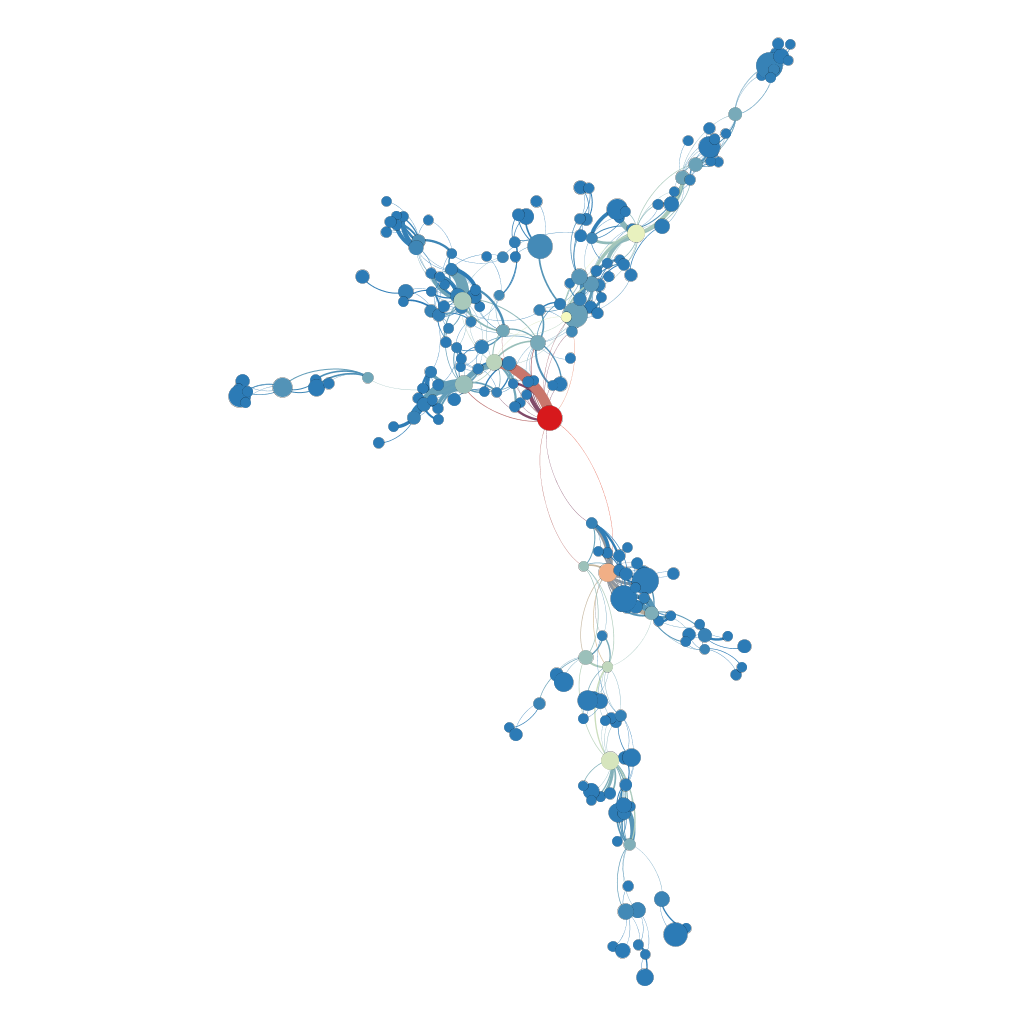
\includegraphics[width=3.41in]{figs/tu_bio_betweenness}

\emph{Notes:}

\begin{itemize}
\tightlist
\item
  214 nodes (18.9\% visible); 615 edges (25.49\% visible).
\item
  \texttt{cluster\_id} with highest betweenness = 43204348; Betweenness
  centrality: 0.50; Total publications = 341; Age = 31
\item
  Name: Harrie H. Weinans; First year: 1987; Last year: 2018
\item
  Google Profile:
  \url{https://scholar.google.com/citations?user=di4NUp8AAAAJ\&hl=en}
\item
  PURE:
  \url{https://pure.tudelft.nl/portal/en/persons/hh-weinans(f31bd75b-1863-4202-b64b-7356538284a7)/publications.html}
\item
  Co-affiliated to UMC Utrecht and TU Delft.
\end{itemize}

\hypertarget{leiden-univ-1}{%
\paragraph{2. Leiden Univ}\label{leiden-univ-1}}

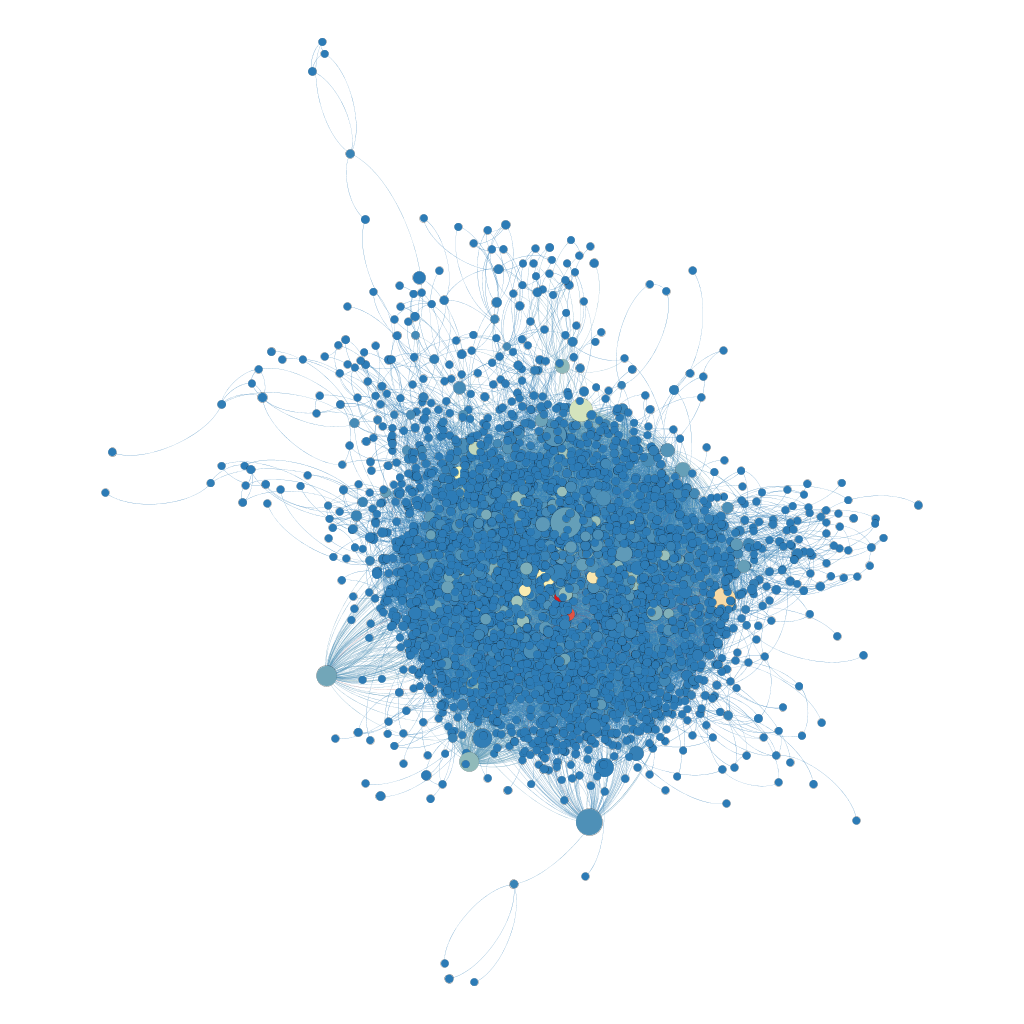
\includegraphics[width=3.41in]{figs/lu_bio_betweenness}

\emph{Notes:}

\begin{itemize}
\tightlist
\item
  Due to the density of the network the selected node can scarcely be
  seen.
\item
  3304 nodes (38.8\% visible); 43647 edges (59.6\% visible).
\item
  \texttt{cluster\_id} with highest betweenness = 19936939; Betweenness
  centrality: 0.47; Total publications = 185; Age = 27
\item
  Name: Ron Wolterbeek; First year: 1991; Last year: 2018
\item
  Institution: \url{https://www.lumc.nl/org/bds/medewerkers/rwolterbeek}
\item
  Affiliated to LUMC.
\end{itemize}

\hypertarget{social-sciences-and-humanities}{%
\subsubsection{Social Sciences and
Humanities}\label{social-sciences-and-humanities}}

\hypertarget{tu-delft-2}{%
\paragraph{1. TU Delft}\label{tu-delft-2}}

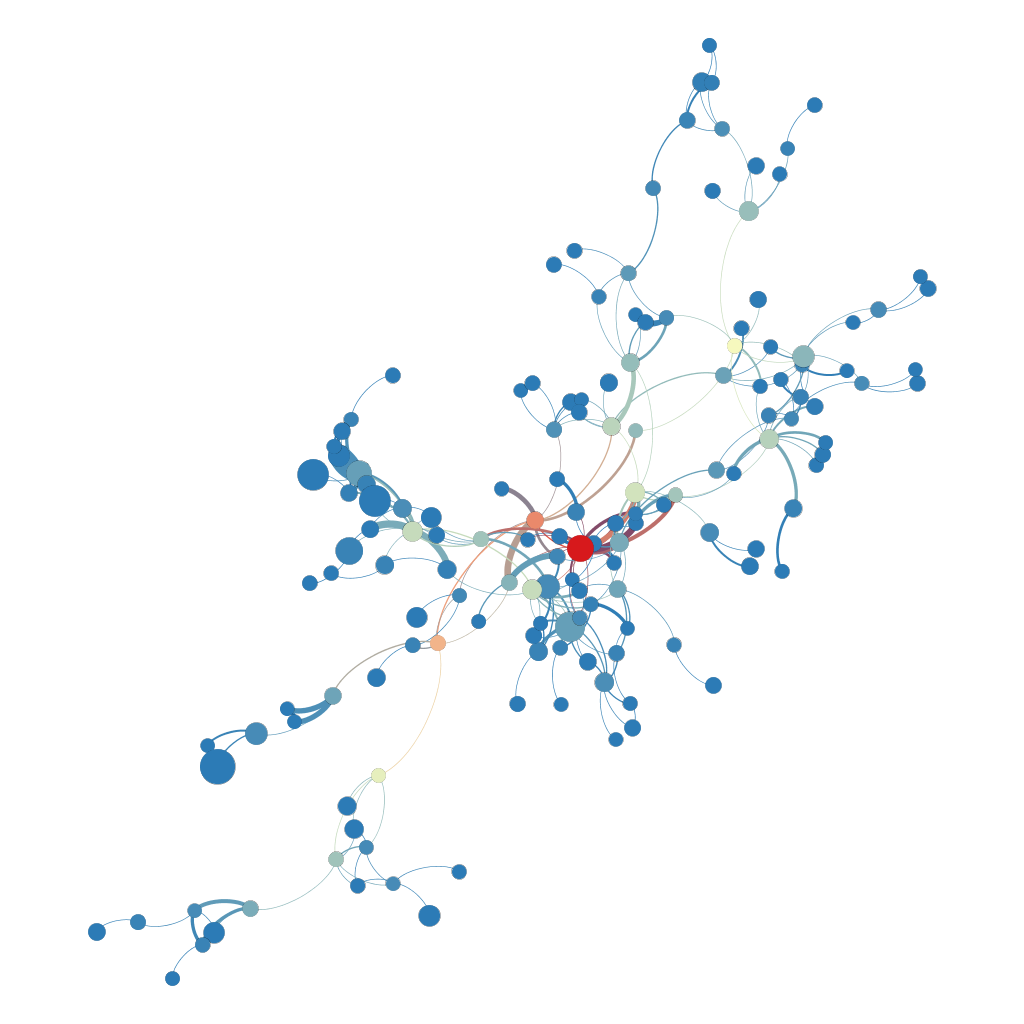
\includegraphics[width=3.41in]{figs/tu_soc_betweenness}

\emph{Notes:}

\begin{itemize}
\tightlist
\item
  151 nodes (12.6\% visible); 281 edges (15.8\% visible).
\item
  \texttt{cluster\_id} with highest betweenness = 12392841; Betweenness
  centrality: 0.41; Total publications = 134; Age = 18
\item
  Name: Bert van Wee; First year: 1999; Last year: 2018
\item
  Google Profile:
  \url{https://scholar.google.es/citations?user=dYUiqMYAAAAJ\&hl=en}
\item
  Institution:
  \url{https://www.tudelft.nl/en/tpm/about-the-faculty/departments/engineering-systems-and-services/people/full-professors/profdr-gp-bert-van-wee/}
\end{itemize}

\hypertarget{leiden-univ-2}{%
\paragraph{2. Leiden Univ}\label{leiden-univ-2}}

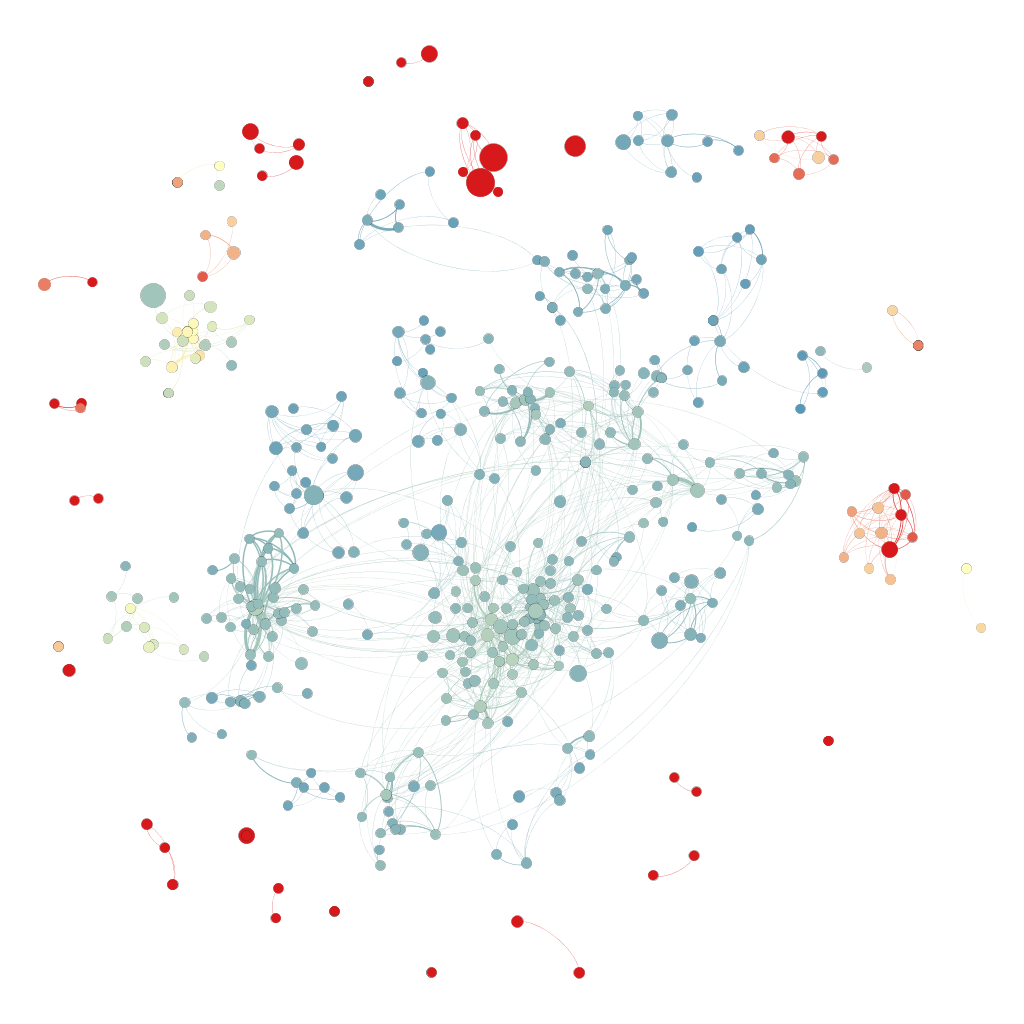
\includegraphics[width=3.41in]{figs/lu_soc_betweenness}

\emph{Notes:}

In this case, the selection of the seed researcher was not based on
network indicator. The network above has the OpenOrd layout (instead of
Yi ) and K-Core=1 group. The main issue here is that this field is
largely populated by biomedical scientists and psychologists and
psychiatrists, fields which are not good representations of Social
Sciences and Humanities. What I have done is looked at those pairs of
scholars with the highest shares of co-authored papers and go down the
list until I found someone who was not from these fields nor from CWTS
(Ludo and Nees are the third pair with more co-authored papers)

\begin{itemize}
\tightlist
\item
  478 nodes (26.5\% visible); 1294 edges (43.1\% visible).
\item
  \texttt{cluster\_id} selected = 36871407; Betweenness centrality:
  0.00; Total publications = 78; Age = 18
\item
  Name: Judi Mesman; First year: 2000; Last year: 2018
\item
  Institution:
  \url{https://www.universiteitleiden.nl/en/staffmembers/judi-mesman/publications\#tab-1}
\item
  Lab1: \url{http://www.diversityinparenting.nl/}
\item
  Lab2: \url{https://www.societalchallengeslab.com/}
\end{itemize}

\hypertarget{expansion-from-seed-to-complete-team}{%
\subsection{Expansion from seed to complete
team}\label{expansion-from-seed-to-complete-team}}

Based on the six individuals selected in the first phase. I know search
for their complete research team. The data retrieval process started on
March, 2019. Here I include for each case how I have proceeded.

\hypertarget{physics-engineering---tu-delft}{%
\subsubsection{Physics \& Engineering - TU
Delft}\label{physics-engineering---tu-delft}}

Dr.~Ir. F.D. Tichelaar belongs to the National Centre for High
Resolution Electron Microscopy. According to its website, he is not the
head of the institute which is formed by 9 researchers (5 staff and 4
researchers and post docs)

\hypertarget{physics-engineering---leiden-univ}{%
\subsubsection{Physics \& Engineering - Leiden
Univ}\label{physics-engineering---leiden-univ}}

Prof.~Ewine van Dishoeck belongs to the Leiden Observatory. According to
its website, there are 179 workers: 33 are staff members, 50 postdocs,
63 PhD students and 26 supporting staff.

\hypertarget{biomedical-sciences---tu-delft}{%
\subsubsection{Biomedical Sciences - TU
Delft}\label{biomedical-sciences---tu-delft}}

Harrie H. Weinans is associate professor at UMC Utrecht in the
department of Orthopaedics and Professor at TU Delft at the
Biomechanical Engineering department. Here information is gathered from
TU Delft. He is a parttime professor. Here I will not include the whole
department, but only researchers working on the Biomaterials \& Tissue
Biomechanics group. Only supporting staff assigned to this group is
included.

\hypertarget{biomedical-sciences---leiden-university}{%
\subsubsection{Biomedical Sciences - Leiden
University}\label{biomedical-sciences---leiden-university}}

Ron Wolterbeek is first-line consultant in the area of Medical
Statistics at LUMC. I could not find him actually in the staff page, so
decided to look into the staff included there. There is not much about
him in the Internet other than his publications.


\end{document}
